\documentclass{article}
\usepackage{float} % Add this package to handle float specifiers
\usepackage[a4paper, top=3cm, bottom=2.5cm, left=2.5cm, right=2.5cm]{geometry} % Ajuste de márgenes
\usepackage[spanish]{babel}
\usepackage[utf8]{inputenc}
\usepackage{tabularx}
\usepackage{tikz}
\usepackage{colortbl}
\usetikzlibrary{mindmap, shapes, positioning}
\usepackage{titling}
\usepackage{graphicx}
\usepackage{fancyhdr}
\usepackage{amsmath}
\usepackage{amssymb}
\usepackage{multicol}
\usepackage{cancel}
\usepackage{pgfplots}
\usepackage{hyperref}
\pgfplotsset{compat=1.18}
\usepackage{titlesec}
\usepackage{tocloft} 
\usepackage{setspace}
\usepackage{forest}

% Configuración de Fancyhdr para encabezados y pies de página
\pagestyle{fancy}
\fancyhf{}
\fancyhead[L]{
\includegraphics[width=2cm]{assets/logo-utp.png}}
\fancyhead[R]{\textit{Administración y organización de empresas.}}

\fancyfoot[R]{\thepage} % Número de página alineado a la derecha

% Ajustes de espaciado entre párrafos y márgenes superiores
\setlength{\parskip}{1.5em}
\setlength{\parindent}{0pt}
\setlength{\headheight}{17.26935pt} % Altura del encabezado
\addtolength{\topmargin}{-2.26935pt} % Compensar el aumento de la altura del encabezado
\setlength{\textheight}{23cm}  % Ajusta el alto del texto

% Definición de comandos personalizados
\newcommand{\SubItem}[1]{
    {\setlength\itemindent{15pt} \item[-] #1}
}

\pagenumbering{gobble}

% Título del documento con mejor control de espaciado
\title{
  
\includegraphics[width=5cm]{./assets/logo-utp.png} \\
  \vspace{1cm}
  \textbf{Universidad Tecnológica del Perú} \\
  \vspace{2cm}
  \textbf{Análisis Estratégico y la Gestión Comercial, Operativa y Corporativa de NVIDIA.} \\
  \vspace{1cm}
  \large \textbf{Para el curso de Administración y organización de empresas.}
}

% Ayerbe Balderrama, Juan Carlos 		U19219954 
% Villanueva Ventura Johan James		U24267335 
% Cuya Javier Katerine Carolina			U24261533 
% Huatay Salcedo Luis Elías					U24218809 
% Dante Daniel Lazo Pamucena				U24266885 

\author{
  \begin{tabular}{ll}
    Ayerbe Balderrama, Juan Carlos 	& U19219954 \\
    Cuya Javier, Katerine Carolina & U24261533 \\
    Huatay Salcedo, Luis Elías & U24218809 \\
    Villanueva Ventura Johan James	& U24267335 \\
  \end{tabular} \\\\
  \texttt{Sección 43925}
}

% ENVIROMENTS

\newenvironment{indexPre}{\begin{center}}{\end{center}}
\newenvironment{introduccion}{\section{Introducción}}{}
\newenvironment{marcoTeorico}{\section{Marco teórico}}{}
\newenvironment{problematica}{\section{Problemática}}{}
\newenvironment{objetivoGeneral}{\section{Objetivo general}}{}
\newenvironment{terminosEstadisticos}{\section{Términos Estadísticos}}{}
\newenvironment{recoleccionDeInformacion}{\section{Recolección de Información}}{}
\newenvironment{metodologia}{\section{Metodología}}{}
\newenvironment{analisisDescriptivo}{\section{Análisis Descriptivo}}{}

\begin{document}
\maketitle

\begin{center}
  Docente. Mg. Sandra Mariana, Flores Ganoza
\end{center}

\restoregeometry

\pagenumbering{arabic} % Numeración arábiga para el resto del documento
\setcounter{page}{2}   % Iniciar numeración en la página 2

\newpage

\tableofcontents

\newpage

\vspace*{\fill}

\begin{introduccion}

  Nvidia es una destacada empresa multinacional con sede en Santa Clara, California, especializada en el diseño y fabricación de unidades de procesamiento gráfico (GPU) para aplicaciones en gaming, inteligencia artificial, visualización profesional y centros de datos. En los últimos años, la empresa ha experimentado un crecimiento significativo, impulsado por su enfoque en la innovación y la calidad de sus productos.

  En este informe, se desarrollará un análisis exhaustivo tanto externo como interno de Nvidia. Utilizaremos herramientas como el análisis PESTEL y FODA para evaluar su entorno. Además, realizaremos un diagnóstico de la gestión comercial de la empresa, identificando sus fortalezas y oportunidades de mejora en áreas clave como marketing, ventas, servicio, personal y retención de talento.

  En cuanto a la gestión operativa y financiera, llevaremos a cabo análisis detallados, incluyendo el balance general de la empresa y la cadena de valor de McKinsey. También se analizará la gestión de TI y la gestión de Investigación y Desarrollo (I+D), con un enfoque especial en la gobernanza y ética de la empresa.
    
\end{introduccion}

\vspace*{\fill}

\newpage

\begin{marcoTeorico}
  \vspace{-0.5cm}
  \subsection{Bussines Model Canvas}

  El Business Model Canvas es una herramienta de gestión estratégica que permite a las empresas describir, diseñar, desafiar, inventar y pivotar su modelo de negocio. Es una plantilla visual con nueve bloques que representan los elementos clave de una empresa, como los segmentos de clientes, las propuestas de valor, los canales de distribución, las relaciones con los clientes, las fuentes de ingresos, los recursos clave, las actividades clave, las asociaciones clave y la estructura de costos.

  Según Sonderegger P. (2020) Un Modelo de Negocio representa a una organización y la manera en la que ésta genera, brinda y crea valor. El Business Model Canvas (Osterwalder, Alexander; Pigneur, Yves, 2013) es una representación innovadora y conceptual que permite visualizar el Modelo de Negocio de una empresa a crear, de la competencia o de cualquier otra organización, permitiendo el análisis y la discusión sobre esto, para poder desarrollar nuevas alternativas estratégicas. 

  \begin{flushright}
    \textit{Sonderegger P. (2020) Cómo utilizar el Business Model Canvas (Lienzo de Modelo de Negocio) para reducir el riesgo}
  \end{flushright}
  \vspace{-0.5cm}
  \subsection{Balance General de una empresa}

El balance general es un estado financiero que muestra la situación patrimonial de una empresa en un momento determinado. Se compone de dos partes: el activo, que representa los bienes y derechos de la empresa, y el pasivo, que refleja las obligaciones y deudas. La diferencia entre el activo y el pasivo es el patrimonio neto, que indica la inversión de los accionistas en la empresa.

Según Altieri D., Martinez E., Perri M. (2018) El Balance General permitirá a los agentes internos comprender la situación actual de la organización, comparándola con la de ejercicios anteriores, y actuará como punto de partida para la proyección de futuras mejoras para la organización (por ejemplo, realización de inversiones para incrementar los flujos u obtener mayores ganancias e ingresos, etc.)

\begin{flushright}
  \textit{Altieri D., Martinez E., Perri M. (2018). Análisis e interpretación de un Balance General}
\end{flushright}
\vspace{-0.5cm}
\subsection{Gestión operativa en una empresa}

La gestión operativa se refiere a la planificación, organización y control de las actividades diarias de una empresa para garantizar su eficiencia y efectividad. Incluye la gestión de recursos humanos, materiales y financieros, así como la implementación de procesos y procedimientos para lograr los objetivos organizacionales.

Según Ccahuay, Jara y Vasquez (2020). Hoy en día en las organizaciones por una mala gestión operativa originan un incremento de costos innecesarios por lo cual se ven afectadas económicamente, por eso las empresas se ven dispuestas a realizar mejoras continuamente para reducir y evitar altos costos logrando tener mejores utilidades e incrementando su competitividad en el mercado.

\begin{flushright}
  \textit{Ccahuay, Jara y Vasquez (2020). Plan de mejora en la gestión operativa para reducir costos de la
  empresa Shalom Empresarial S.A.C. Chiclayo.}
\end{flushright}



  \subsection{Marketing Mix, las 4 P's}

  Las 4 P's del marketing mix son un conjunto de variables que las empresas pueden controlar para influir en la demanda de sus productos o servicios. Las 4 P's son:
  
  \begin{itemize}
    \item \textbf{Producto:} Se refiere a los bienes o servicios que la empresa ofrece a sus clientes. Nvidia ofrece una amplia gama de productos, desde tarjetas gráficas para gaming hasta soluciones de cómputo de alto rendimiento para centros de datos.
    \item \textbf{Precio:} Se refiere al valor monetario que los clientes están dispuestos a pagar por los productos o servicios de la empresa. Nvidia utiliza una estrategia de precios premium para sus productos de alta gama, basada en su calidad y rendimiento.
    \item \textbf{Plaza:} Se refiere a los canales de distribución que la empresa utiliza para llevar sus productos o servicios al mercado. Nvidia vende sus productos a través de distribuidores autorizados, tiendas en línea y socios comerciales.
    \item \textbf{Promoción:} Se refiere a las estrategias de comunicación que la empresa utiliza para dar a conocer sus productos o servicios y persuadir a los clientes a comprarlos. Nvidia utiliza una combinación de publicidad, relaciones públicas y marketing digital para promocionar sus productos.
  \end{itemize}

  Según Paucar J. (2019), El Marketing Mix es un conjunto de decisiones sobre producto precio, canales de distribución y comunicaciones (o promoción) con las que se despliega la estrategia de marketing. También llamadas las 4 P del marketing por sus siglas en inglés y sus componentes están interrelacionados.

  \begin{flushright}
    \textit{Paucar J. (2019) Evolución de las 4P´s o Marketing Mix.}
  \end{flushright}  

  \subsection{Gestión de Ventas}

  La gestión de ventas es el proceso de planificar, organizar, dirigir y controlar las actividades de ventas de una empresa para alcanzar sus objetivos comerciales. La gestión de ventas implica la identificación de oportunidades de venta, la prospección de clientes, la presentación de propuestas comerciales, el cierre de ventas y el seguimiento postventa.

  Según Rojas Z. (2017). La gestión de ventas es muy importante en el desarrollo, crecimiento y continuidad de
  las empresas de cualquier sector de empresarial, sea comercial, de servicios, industrial,
  etc. El planificar la gestión de ventas y costos es indispensable para establecer las guías
  de acciones necesarias para poder obtener una buena rentabilidad durante el ejercicio
  fiscal.

  \begin{flushright}
    \textit{  Rojas Z. (2017) La Gestión de Ventas y Rentabilidad.}
  \end{flushright}

\newpage
  \subsection{Gestión del servicio}

  La gestión del servicio es el proceso de planificar, organizar, dirigir y controlar las actividades de servicio al cliente de una empresa para garantizar la satisfacción del cliente y la fidelización. La gestión del servicio implica la atención al cliente, la resolución de problemas, la gestión de reclamos y la mejora continua de la calidad del servicio.

  Según  Piñeiro A. Varela J. Rail A. (2006), Partiendo de la importancia y la valoración que los usuarios otorgan a cada uno de los atributos relevantes de un servicio,es posible obtener una herramienta en los que se incluyan recomendacionespara la gestión de los recursos organizacionales. Sin embargo, esta herramienta ha estado sujeta a controversias desde sus orígenes.

  \begin{flushright}
    \textit{ Piñeiro A. Varela J. Rail A. (2006) El análisis de importancia-valoración aplicado a la gestión de servicios}
  \end{flushright}

  \subsection{Gestión del personal}

    La gestión del personal es el proceso de planificar, organizar, dirigir y controlar las actividades relacionadas con el personal de una empresa para garantizar su eficiencia y productividad. La gestión del personal implica la selección, contratación, capacitación, evaluación y desarrollo del personal, así como la gestión de las relaciones laborales y la prevención de conflictos.

    Según Hernández A. (2006), Un verdadero sistema de provisión de empleos de carrera debe caracterizarse por la consonancia que exista entre el diseño normativo y la aplicación práctica que de él se haga, pues poco será el aporte de 
    un conjunto regulatorio armónico, coherente, ágil y moderno en esta materia si la realidad 
    administrativa no concuerda con tales postulados.

    \begin{flushright}
      \textit{Hernández A. (2006) La provisión de empleos de carrera en Colombia: lineamientos de un nuevo modelo de gestión de personal en el sector público}
    \end{flushright}

\end{marcoTeorico}

\newpage
\begin{objetivoGeneral}
  \vspace{-0.7cm}
  Realizar un diagnóstico integral de la empresa Nvidia, abarcando las áreas de gestión comercial, operativa, financiera y de TI. Este diagnóstico incluirá la identificación de fortalezas y oportunidades de mejora en marketing, ventas, servicio, personal y retención de talento. Además, se llevará a cabo un análisis externo e interno utilizando herramientas como el análisis PESTEL, el modelo de las 5 fuerzas de Porter, la evaluación de la cadena de valor y la construcción de una matriz FODA. Este enfoque permitirá comprender tanto el entorno macroeconómico como los factores internos de la empresa, facilitando la toma de decisiones estratégicas informadas para maximizar su posición competitiva en el mercado. También se analizará la gestión de TI con un enfoque en la optimización de la eficiencia, la investigación y desarrollo, y el gobierno corporativo, destacando las prácticas fundamentales para el buen funcionamiento de la empresa.
  \vspace{-0.7cm}
  \subsection{Objetivos específicos}
  \vspace{-0.5cm}
  \begin{multicols}{2}
    \begin{enumerate}
      \item \textbf{Descripción de la empresa:} Describir la estructura organizacional, los productos y servicios ofrecidos, y los mercados en los que opera Nvidia.
      \item \textbf{Análisis estratégico:} Realizar un análisis estratégico de Nvidia, esto incluye un análisis externo e interno de la empresa.
      \item \textbf{Análisis externo:} Realizar un análisis PESTEL para identificar los factores políticos, económicos, sociales, tecnológicos, ecológicos y legales que afectan a Nvidia.
      \subitem Aplicar el modelo de las 5 fuerzas de Porter para evaluar la competencia y las dinámicas del mercado.
      \item \textbf{Análisis interno:} Evaluar los recursos y capacidades internas de Nvidia, incluyendo su estructura organizacional, cultura corporativa y capacidades tecnológicas.
      \item \textbf{Matriz FODA:} Construir una matriz FODA (Fortalezas, Oportunidades, Debilidades, Amenazas) para identificar las áreas clave de mejora y las oportunidades estratégicas.
      \item \textbf{Desarrollo del Business Model Canvas:} Desarrollar un Business Model Canvas para visualizar y analizar el modelo de negocio de Nvidia, identificando sus componentes clave y áreas de mejora.
      \item \textbf{Análisis Financiero} Analizar los estados financieros de Nvidia, incluyendo su Balance General para comprender su situación financiera analizando los pricipales indicadores.
      \item \textbf{Cadena de valor:} Aplicar la cadena de valor de McKinsey para evaluar las actividades clave de Nvidia y su contribución al valor total, con un enfoque en la ventaja competitiva.
      \item \textbf{Gestión operativa:} Evaluar la planificación y monitoreo de la gestión operativa de Nvidia, examinando los principales indicadores que influyen en su desempeño operativo.
      \item \textbf{Gestión comercial:} Analizar la gestión del marketing de Nvidia, evaluando su estrategia de producto, precio, plaza y promoción.
      \item \textbf{Gestión de ventas:} Evaluar la gestión de ventas de Nvidia, identificando sus procesos de prospección, presentación, cierre y seguimiento de ventas.
      \item \textbf{Gestión del servicio al cliente:} Analizar la gestión del servicio al cliente de Nvidia, evaluando su atención al cliente, resolución de problemas y gestión de reclamos.
      \item \textbf{Gestión del personal:} Evaluar la gestión del personal de Nvidia, identificando sus procesos de selección, contratación, capacitación, evaluación y desarrollo del personal.
      \item \textbf{Gestión de TI:} Analizar la gestión de TI de Nvidia, con un enfoque en la optimización de la eficiencia, la investigación y desarrollo, y el gobierno corporativo.
      \item \textbf{Gestión de I+D:} Evaluar la gestión de Investigación y Desarrollo de Nvidia, identificando sus procesos de innovación, colaboración y protección de la propiedad intelectual.
      \item \textbf{Gobernanza corporativa:} Analizar la gobernanza corporativa de Nvidia, evaluando su control interno, la gestión de regiesgos la responsabilidad social y la sostenibilidad ambiental.
      \item \textbf{Conclusiones y recomendaciones:} Resumir los hallazgos del análisis y proporcionar recomendaciones para mejorar la posición competitiva de Nvidia en el mercado.
    \end{enumerate}    
  \end{multicols}
\end{objetivoGeneral}

\newpage

\section{Descripción de la empresa: Nvidia}

Nvidia es una empresa multinacional con sede en Santa Clara, California, especializada en el diseño y fabricación de unidades de procesamiento gráfico (GPU) para aplicaciones en gaming, inteligencia artificial, visualización profesional y centros de datos. Fundada en 1993 por Jensen Huang, Chris Malachowsky y Curtis Priem, Nvidia ha experimentado un crecimiento significativo en los últimos años, convirtiéndose en un líder en el mercado de tecnología y semiconductores..

Fundada en 1993 por Jensen Huang, Nvidia se ha convertido en una empresa líder en software y hardware de procesamiento gráfico y AI. Especializada en el diseño de GPUs, APIs para computación de alto rendimiento y SoCs para dispositivos móviles y automóviles, Nvidia ha transformado industrias como arquitectura, medios, entretenimiento, automoción, investigación y diseño de manufactura. En 2006, la compañía hizo sus chips programables, permitiendo su uso en aplicaciones más allá de los videojuegos y capitalizando el auge de la inteligencia artificial. Hoy, Nvidia es una de las pocas empresas con un valor de mercado superior al billón de dólares, junto a gigantes como Apple, Microsoft, Alphabet y Amazon.

\subsection{Visión:}

Nvidia busca liderar la revolución de la IA y la computación en GPU,
transformando industrias mediante tecnologías que aceleren la innovación y
definan el futuro.

\subsection{Misión:}

Resolver algunos de los problemas tecnológicos más desafiantes del
mundo, desde videojuegos hasta exploración científica, con un equipo de
talento excepcional.

\subsection{Valores:}

\begin{itemize}
  \item \textbf{Innovación:} Desarrollo de tecnologías de vanguardia en AI y computación.
  \item \textbf{Excelencia:} Compromiso con productos de alta calidad.
  \item \textbf{Colaboración:} Fomento del trabajo en equipo y la cooperación.
  \item \textbf{Integridad:} Operar con ética y responsabilidad.
  \item \textbf{Diversidad e Inclusión:} Valorar perspectivas diversas para fomentar la innovación.
  \item \textbf{Responsabilidad Social:} Compromiso con la sostenibilidad y el impacto positivo en las comunidades.
\end{itemize}

Estos principios guían las decisiones y estrategias de Nvidia, manteniendo su éxito global.

\newpage

\section{Análisis estratégico: Externo}

El presente cuadro es el análisis PESTEL de macroentorno que afecta a Nvidia. Este análisis se centra en los factores políticos, económicos, sociales, tecnológicos, ecológicos y legales que influyen en la empresa y en su entorno operativo.

\begin{table}[h!]
  \centering
  \renewcommand{\arraystretch}{1.5}
  \setlength{\tabcolsep}{10pt}
  \begin{tabular}{|p{4.5cm}|p{4.5cm}|p{4.5cm}|}
    \hline
    \textbf{Político} & \textbf{Económico} & \textbf{Socioculturales} \\ \hline
    Estabilidad política & Crecimiento económico & Adopción de tecnología \\ 
    Regulaciones de mercado & Inflación & Educación y formación \\ 
    Incentivos a la tecnología & Tipo de cambio & Cultura de innovación \\ 
    Regulaciones de protección de datos & Política Fiscal & Acceso a tecnología \\ 
    & Competencia Local & Ingresos y poder adquisitivo \\ \hline
    \textbf{Tecnológicos} & \textbf{Ecológicos} & \textbf{Legales} \\ \hline
    Desarrollo de infraestructura tecnológica & Regulaciones ambientales & Regulaciones de protección de datos \\ 
    Innovación & Sostenibilidad y responsabilidad ambiental & Leyes de propiedad intelectual \\ 
    Tendencia del desarrollo tecnológico & Eficiencia energética & Normativas laborales \\ 
    Ecosistema tecnológico global & Cambio climático & Regulaciones en aranceles \\ 
    Tecnologías emergentes & Certificaciones ambientales & Cumplimiento regulatorio \\ \hline
  \end{tabular}
  \caption{Análisis PESTEL de Nvidia}
  \label{tab:PESTEL}
\end{table}

\section{5 Fuerzas de Porter: Microentorno}

Las 5 fuerzas de Porter son un modelo de análisis competitivo que permite evaluar la competencia y las dinámicas del mercado en el que opera una empresa. Las 5 fuerzas son: competencia en la industria, poder de negociación de los proveedores, poder de negociación de los compradores, amenaza de productos sustitutos y amenaza de nuevos competidores.

\subsection{Rivalidad entre competidores}

\textbf{\large{Alto:}} Nvidia compite intensamente contra las empresas Amd e Intel en el mercado
de procesadores gráficos (GPUS) de alto rendimiento y optimización tecnológica. La
competencia se centra en ofrecer productos de mejor calidad-precio para atraer
consumidores lo que impulsa la innovación y obliga a ajustar las estrategias de
precios para preservar y expandir su cuota de mercado.

\subsection{Poder de negociación de los proveedores}

\textbf{\large{Bajo:}} La empresa Nvidia negocia con muchos proveedores que se encuentran a su
disposición tanto nacional como internacional, por lo cual tiene por elegir entre
calidad y precios de los productos o componentes para la elaboración de sus
tarjetas gráficas.

\subsection{Poder de negociación de los clientes}

\textbf{\large{Medio:}} Los consumidores peruanos pueden acceder a productos Nvidia, pero
los costos de importación, impuestos y disponibilidad limitada influyen en sus
opciones. Aunque buscan calidad y precio, la competencia directa es
limitada, con AMD como principal alternativa. Sin embargo,
la fuerte
presencia de Nvidia y su reputación en el mercado de alto rendimiento
disminuyen el poder de negociación de los clientes.

\subsection{Amenaza de nuevos entrantes}

\textbf{\large{Baja:}} Es poco probable que nuevas empresas ingresen al mercado de GPUs
en Perú debido a las altas barreras de entrada, como la inversión en
tecnología y el conocimiento especializado. Nvidia enfrenta poca amenaza en
este aspecto, ya que los posibles nuevos competidores, tanto locales como
internacionales, no tienen el mismo nivel de recursos ni la capacidad para
competir en calidad. AMD e Intel, sus principales rivales, ya están
consolidados, lo que hace que los nuevos entrantes sean poco comunes.

\subsection{Amenaza de productos sustitutos}

\textbf{\large{Medio:}} En Perú, los principales productos sustitutos podrían ser GPUs integradas en
procesadores de Intel o AMD, así como soluciones en la nube para algunas
aplicaciones. Sin embargo, estos sustitutos no ofrecen el mismo nivel de
rendimiento que las GPUs dedicadas de Nvidia, lo que reduce su amenaza en
mercados como el de los videojuegos o aplicaciones gráficas avanzadas.

\newpage

\section{Análisis interno}

El análisis interno de Nvidia se centra en evaluar los recursos y capacidades internas de la empresa, incluyendo su estructura organizacional, cultura corporativa y capacidades tecnológicas. Este análisis permite identificar las fortalezas y debilidades de la empresa, así como las oportunidades y amenazas que enfrenta en su entorno operativo.

\subsection{Cadena de valor de Nvidia}

Es una herramienta de análisis que permite identificar las actividades clave de una empresa y su contribución al valor total. La cadena de valor de Nvidia se divide en actividades primarias y actividades de soporte, que incluyen:

\begin{center}
  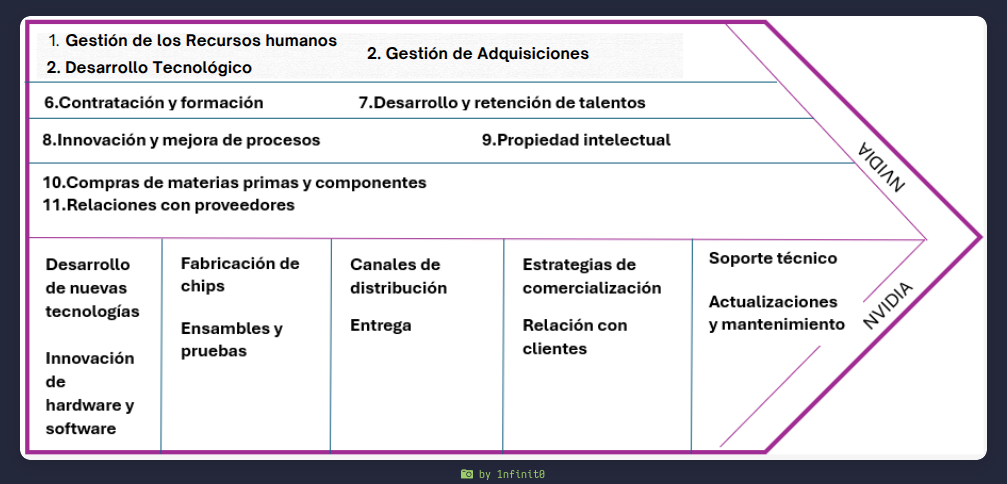
\includegraphics[width=15cm]{./assets/cadenadevalor.png}
\end{center}

\section{Matriz FODA}

Los factores clave de éxito de Nvidia se basan en su capacidad para innovar y liderar en tecnologías emergentes como la inteligencia artificial, la computación en la nube y la conducción autónoma. La empresa ha demostrado una sólida trayectoria de crecimiento y rentabilidad, respaldada por su enfoque en la calidad y el rendimiento de sus productos. Sin embargo, Nvidia también enfrenta desafíos en áreas como la competencia, la regulación y la sostenibilidad ambiental.

La matriz FODA es una herramienta de análisis estratégico que permite identificar las fortalezas, oportunidades, debilidades y amenazas de una empresa. La matriz FODA de Nvidia se presenta a continuación:

\begin{table}[ht!]
  \centering
  \renewcommand{\arraystretch}{1.5}
  \setlength{\tabcolsep}{5pt}
  \begin{tabular}{|p{6cm}|p{6cm}|}
    \hline
    \textbf{Fortalezas} & \textbf{Debilidades} \\ \hline
    Liderazgo en Innovación & Dependencia del mercado de GPUs \\ 
    Portafolio diversificado & Altos costos de Investigación \\ 
    Marca reconocida & Problemas de suministro \\ 
    Desarrollo de tecnologías avanzadas & \\ \hline
    \textbf{Oportunidades} & \textbf{Amenazas} \\ \hline
    Crecimiento en inteligencia artificial & Competencia intensa \\ 
    Expansión de nuevos mercados & Cambios en la regulación \\ 
    Desarrollo de tecnologías emergentes & Ciclos económicos (los problemas de reseción e inflación) \\ 
    Adquisiciones estratégicas & Riesgos tecnológicos \\ \hline
  \end{tabular}
  \caption{Matriz FODA de Nvidia}
  \label{tab:FODA}
\end{table}

\section{Bussines Model Canvas}

El Business Model Canvas de Nvidiamuestra los nueve bloques clave que describen su modelo de negocio. Este modelo se basa en la innovación tecnológica y la calidad de sus productos, con un enfoque en la diversificación y la expansión a nuevos mercados.

Desarrollado por Alexander Osterwalder y Yves Pigneur, el Business Model Canvas es una herramienta de gestión estratégica que permite a las empresas describir, diseñar, desafiar, inventar y pivotar su modelo de negocio. El Business Model Canvas de Nvidia se presenta a continuación:

\begin{center}
  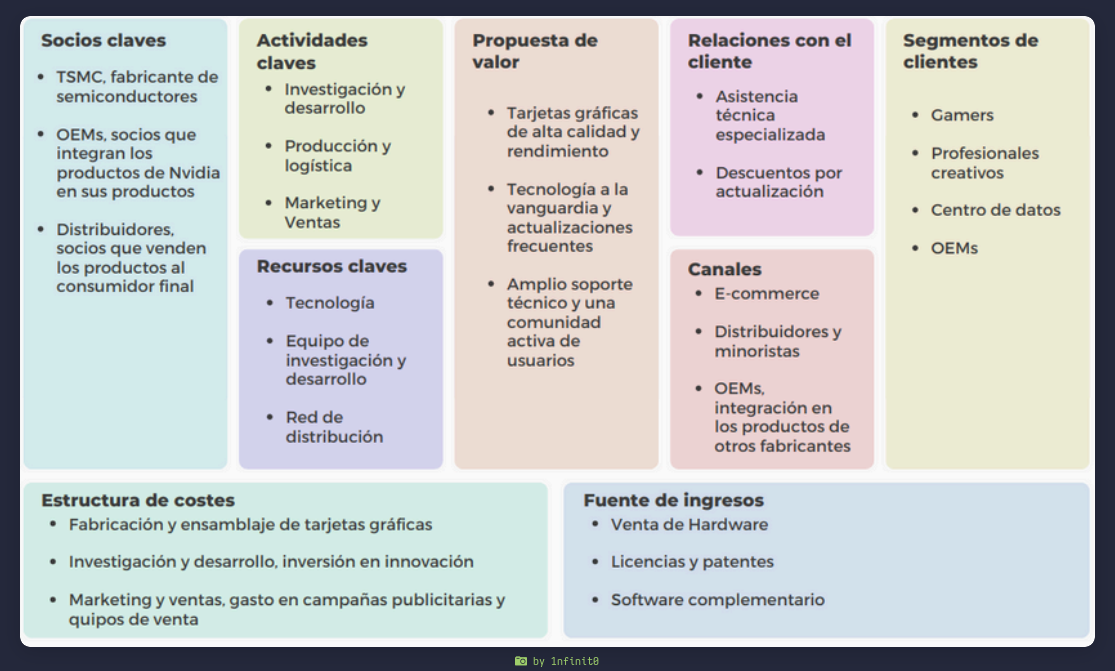
\includegraphics[width=15cm]{./assets/canva.png}
\end{center}

\section{Reflecciones sonre el análisis interno y externo}

El análisis interno y externo de Nvidia revela una serie de fortalezas y oportunidades, así como debilidades y amenazas que la empresa enfrenta en su entorno operativo. Las fortalezas de Nvidia incluyen su liderazgo en innovación, su portafolio diversificado y su marca reconocida. Sin embargo, la empresa también enfrenta desafíos como la competencia intensa, los cambios en la regulación y los riesgos tecnológicos. Para mantener su posición competitiva en el mercado, Nvidia debe capitalizar sus fortalezas y oportunidades, al tiempo que aborda sus debilidades y amenazas. Esto requiere un enfoque estratégico en áreas clave como la innovación, la diversificación y la expansión a nuevos mercados, así como la gestión eficiente de los riesgos y la regulación.

\section{Contabilidad financiera de NVIDIA}

La contabilidad financiera de Nvidia se basa en la presentación de informes financieros precisos y transparentes que reflejen la situación financiera de la empresa. Los estados financieros de Nvidia incluyen el balance general, el estado de resultados y el estado de flujos de efectivo, que proporcionan información detallada sobre los activos, pasivos, ingresos y gastos de la empresa. El análisis de los estados financieros de Nvidia permite evaluar su desempeño financiero, identificar áreas de mejora y tomar decisiones estratégicas informadas.

Algunos aspectos clave para el desarrollo de la contabilidad financiera de Nvidia incluyen:

% Activo no corriente: Nvidia posee activos no corrientes como propiedades, planta y equipo,
% inversiones a largo plazo y otros activos intangibles que contribuyen a su capacidad productiva y
% competitiva a largo plazo.
% Activo corriente: Los activos corrientes de Nvidia incluyen efectivo, inversiones a corto plazo,
% cuentas por cobrar y otros activos l´ıquidos que respaldan sus operaciones diarias y financian sus
% necesidades a corto plazo.
% Patrimonio neto: El patrimonio neto de Nvidia representa la inversi´on de los accionistas en la
% empresa y refleja su participaci´on en los activos y pasivos de la misma.
% Pasivo no corriente: Nvidia tiene pasivos no corrientes como deudas a largo plazo, arrendamientos
% financieros y otras obligaciones a largo plazo que financian sus inversiones a largo plazo.
% Pasivo corriente: Los pasivos corrientes de Nvidia incluyen cuentas por pagar, deudas a corto
% plazo y otras obligaciones que deben ser pagadas en el corto plazo.

\begin{itemize}
  \item \textbf{Activos no corrientes:} Nvidia posee activos no corrientes como propiedades, planta y equipo, inversiones a largo plazo y otros activos intangibles que contribuyen a su capacidad productiva y competitiva a largo plazo.
  \item \textbf{Activos corrientes:} Los activos corrientes de Nvidia incluyen efectivo, inversiones a corto plazo, cuentas por cobrar y otros activos líquidos que respaldan sus operaciones diarias y financian sus necesidades a corto plazo.
  \item \textbf{Patrimonio neto:} El patrimonio neto de Nvidia representa la inversión de los accionistas en la empresa y refleja su participación en los activos y pasivos de la misma.
  \item \textbf{Pasivo no corriente:} Nvidia tiene pasivos no corrientes como deudas a largo plazo, arrendamientos financieros y otras obligaciones a largo plazo que financian sus inversiones a largo plazo.
  \item \textbf{Pasivo corriente:} Los pasivos corrientes de Nvidia incluyen cuentas por pagar, deudas a corto plazo y otras obligaciones que deben ser pagadas en el corto plazo.
\end{itemize}

Un ejemplo del balance general de NVIDIA en el rango 2020-2021 se muestra a continuación:

%imagen:

\begin{center}
  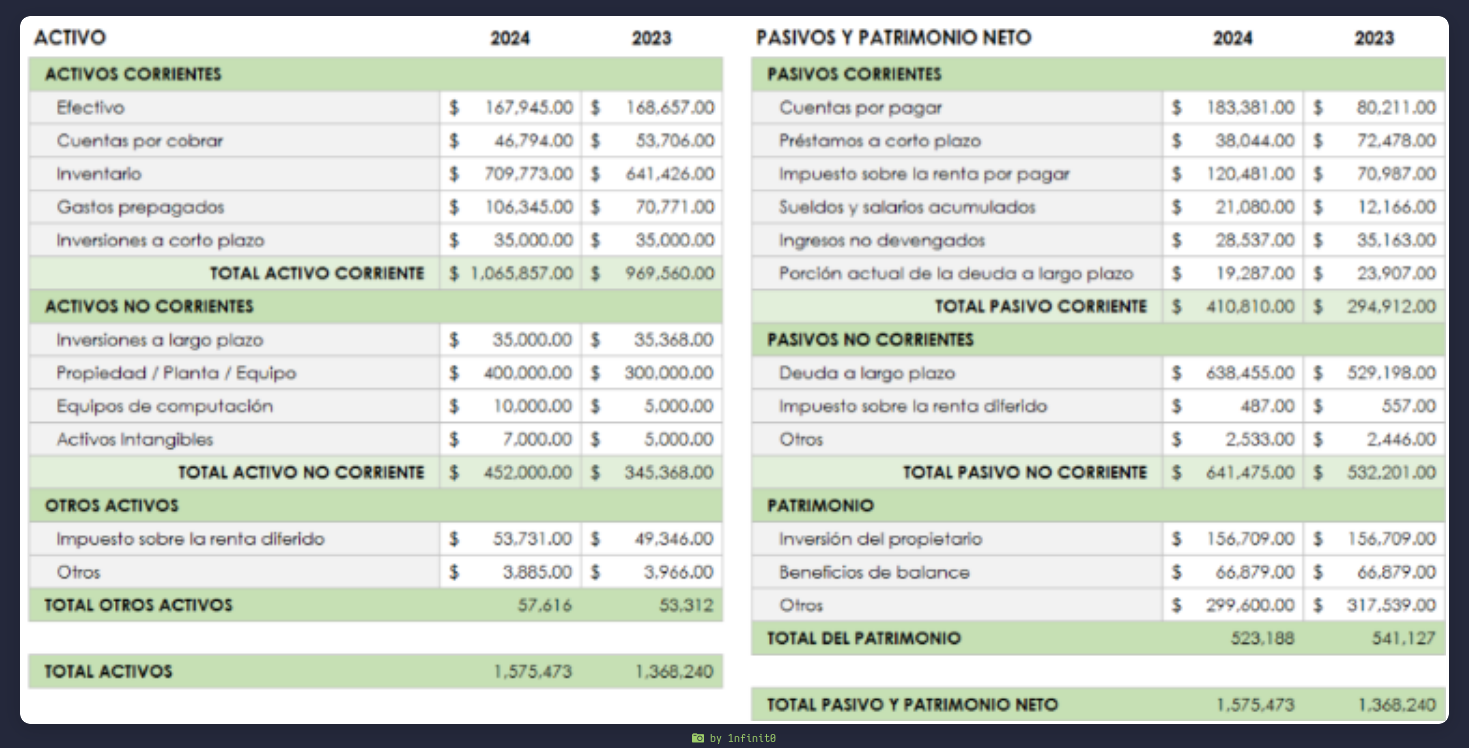
\includegraphics[width=15cm]{./assets/financiero.png}
  \textit{Balance General de Nvidia 2020-2021}
\end{center}

\begin{center}
  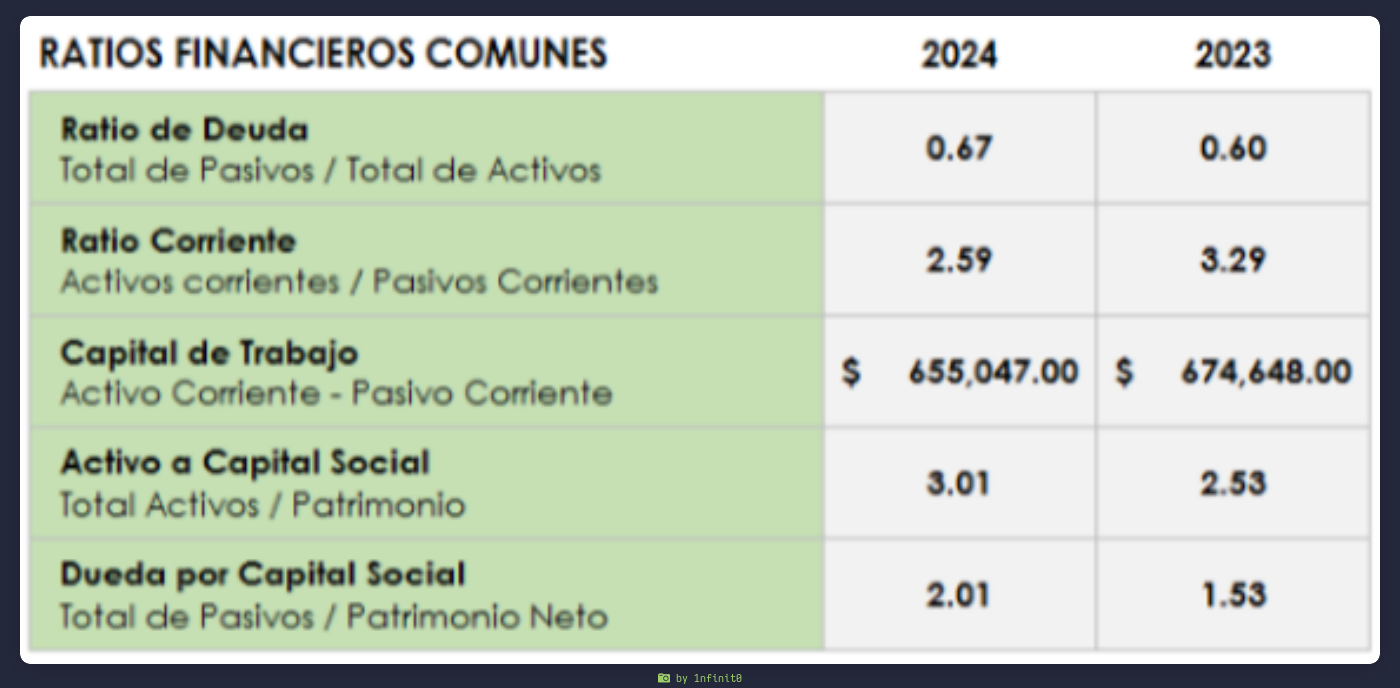
\includegraphics[width=15cm]{./assets/f2.png}
  \textit{Balance General de Nvidia 2020-2021}
\end{center}

\newpage
\section{Estado de resultados:}

El estado de resultados, también conocido como estado de ganancias y pérdidas, es un reporte financiero que muestra de manera detallada la situación de la empresa, es decir, si obtuvo ganancias o pérdidas durante un ciclo contable.

\begin{center}
  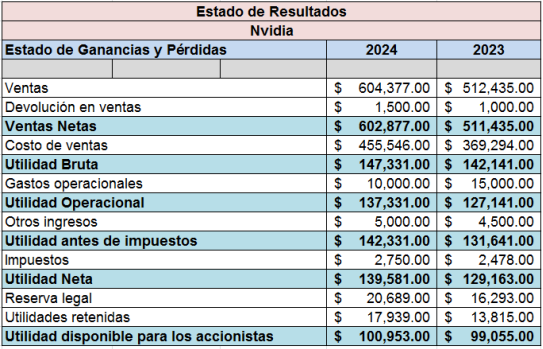
\includegraphics[width=15cm]{./assets/estado_resultados.png}
  \textit{Estado de resultados de Nvidia 2020-2021}
\end{center}

\section{Indicadores de la gestion financiera}

\begin{itemize}
  \item \textbf{Ratios de Liquidez:} Los ratios de liquidez de Nvidia, como la liquidez corriente, evalúan su capacidad para cumplir con sus obligaciones a corto plazo y su solvencia financiera. Los ratios de liquidez se pueden calcular de la siguiente manera:
  \begin{itemize}
    \item \textbf{Ratio de Liquidez Corriente:} \(\text{Liquidez Corriente} = \frac{\text{Activo Corriente}}{\text{Pasivo Corriente}}\)
    \item \textbf{Ratio de Liquidez Rápida:} \(\text{Liquidez Rápida} = \frac{\text{Activo Corriente} - \text{Inventarios}}{\text{Pasivo Corriente}}\)
  \end{itemize}

  \item \textbf{Ratios de Rentabilidad:} Los ratios de rentabilidad miden la capacidad de Nvidia para generar beneficios a partir de sus ventas y activos. Algunos de los ratios de rentabilidad incluyen:
  \begin{itemize}
    \item \textbf{Margen de Beneficio Neto:} \(\text{Margen de Beneficio Neto} = \frac{\text{Beneficio Neto}}{\text{Ventas Netas}} \times 100\)
    \item \textbf{Rentabilidad sobre Activos (ROA):} \(\text{ROA} = \frac{\text{Beneficio Neto}}{\text{Total Activos}} \times 100\)
    \item \textbf{Rentabilidad sobre Patrimonio (ROE):} \(\text{ROE} = \frac{\text{Beneficio Neto}}{\text{Patrimonio Neto}} \times 100\)
  \end{itemize}

\newpage

  \item \textbf{Ratios de Endeudamiento:} Los ratios de endeudamiento evalúan la estructura de capital de Nvidia y su capacidad para cumplir con sus obligaciones de deuda. Algunos de los ratios de endeudamiento incluyen:
  \begin{itemize}
    \item \textbf{Ratio de Deuda Total:} \(\text{Ratio de Deuda Total} = \frac{\text{Total Pasivos}}{\text{Total Activos}} \times 100\)
    \item \textbf{Ratio de Deuda a Patrimonio:} \(\text{Ratio de Deuda a Patrimonio} = \frac{\text{Total Pasivos}}{\text{Patrimonio Neto}}\)
  \end{itemize}

  \item \textbf{Ratios de Eficiencia:} Los ratios de eficiencia miden la eficacia con la que Nvidia utiliza sus activos y gestiona sus operaciones. Algunos de los ratios de eficiencia incluyen:
  \begin{itemize}
    \item \textbf{Rotación de Inventarios:} \(\text{Rotación de Inventarios} = \frac{\text{Costo de Ventas}}{\text{Inventarios Promedio}}\)
    \item \textbf{Rotación de Activos:} \(\text{Rotación de Activos} = \frac{\text{Ventas Netas}}{\text{Total Activos}}\)
  \end{itemize}
  
\end{itemize}

\section{Cadena de valor de McKinsey}

El modelo de McKinsey mezcla las funciones internas de la empresa y la visión global del sector, definiendo el “sistema de negocio”. Para utilizar esta herramienta debemos clasificar dentro de las siguientes columnas aquellos factores que definan la ventaja competitiva de la empresa. Estas columnas incluyen factores necesarios para satisfacer al cliente, aquellos que nos diferencian de la competencia y los que más contribuyen a la formación de valor para la empresa.

A continuación se presenta la cadena de valor de McKinsey de Nvidia:

\begin{center}
  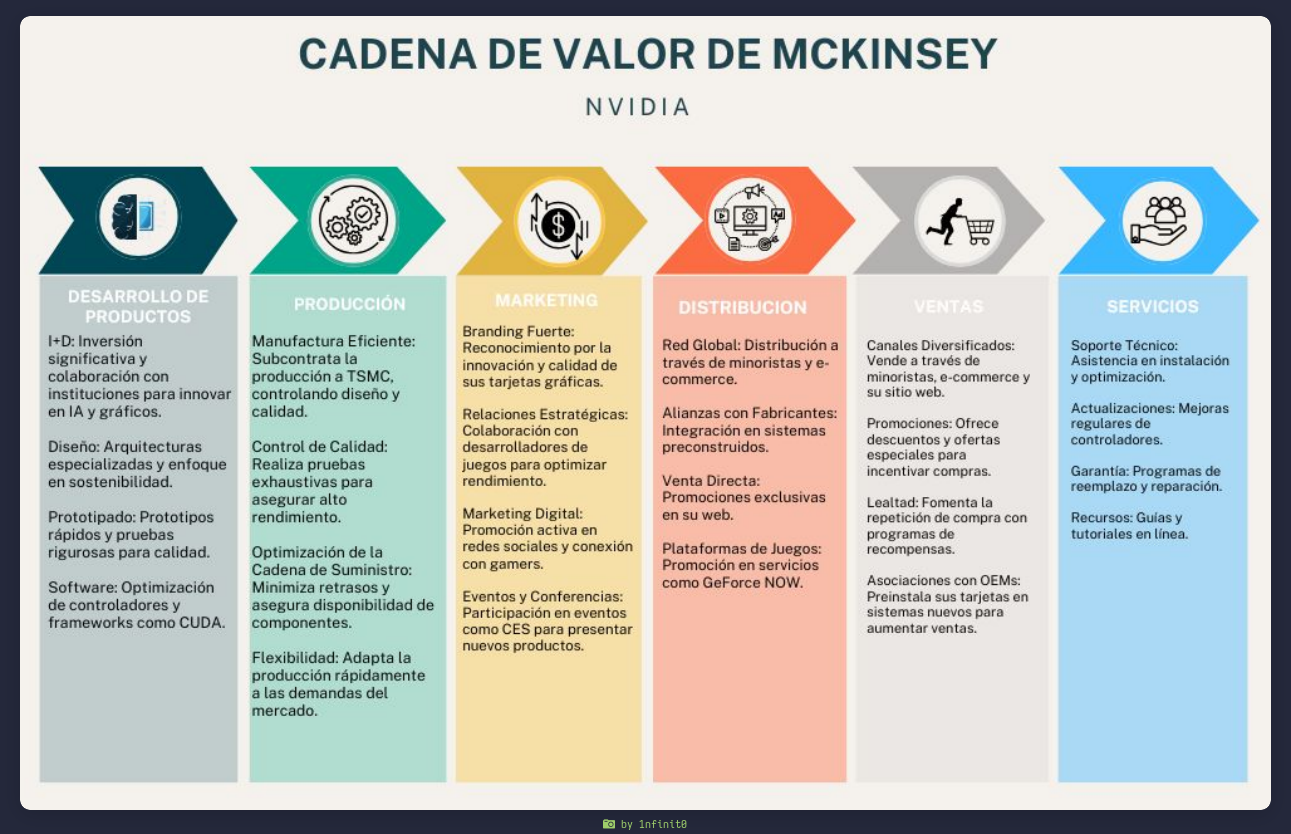
\includegraphics[width=15cm]{./assets/mckenzy.png}
\end{center}

\section{Planificación de la gestión operativa}

La planificación de la gestión operativa de Nvidia se centra en la optimización de los procesos y recursos para garantizar la eficiencia y la calidad en la producción y distribución de sus productos. La empresa utiliza herramientas de gestión de la calidad y la productividad para mejorar continuamente sus operaciones y satisfacer las necesidades de sus clientes.

\subsection{Plan operativo anual (POA)}

El POA es un documento que detalla las metas y objetivos operativos de la empresa para el próximo año, así como las acciones y recursos necesarios para alcanzarlos. El POA debe estar alineado con el plan estratégico de la empresa y contener indicadores de gestión para monitorear su cumplimiento.

\begin{enumerate}
  \item \textbf{Plan estratégico:} Necesitaremos la visión de la empresa además de las estrategias y objetivos a largo plazo.
  \begin{itemize}
    \item \textbf{Visión:} Ser líder en el mercado de tarjetas gráficas y soluciones de cómputo de alto rendimiento para el año 2026.
    \item \textbf{Estrategias:} Desarrollar nuevas GPU con mayor rendimiento y eficiencia energética, expandir la presencia en mercados emergentes y fortalecer la relación con los socios comerciales.
  \end{itemize}
  
  \item \textbf{Reducción del alcance:} Se limita el desarrollo de la estrategia al área de investigación y desarrollo de nuevas GPU.
  
  \item \textbf{Identificación de los participantes:} Se asignan responsabilidades a los equipos de investigación y desarrollo, incluyendo científicos, ingenieros y diseñadores.
  
  \item \textbf{Creación del plan operativo:} Las acciones que se llevarán a cabo incluyen la investigación de nuevas tecnologías, el diseño de prototipos y la realización de pruebas de rendimiento.
  
  \item \textbf{Medición del éxito:} Se utilizarán indicadores de gestión como el tiempo de desarrollo, el rendimiento de las nuevas GPU y la satisfacción del cliente.
\end{enumerate}

A continuación de muestra un ejemplo de un POA para Nvidia:

\begin{table}[H]
  \centering
  \renewcommand{\arraystretch}{1.5}
  \setlength{\tabcolsep}{4pt}
  \begin{tabular}{|p{2.3cm}|p{2cm}|p{3.2cm}|p{1.8cm}|p{3.5cm}|p{2.5cm}|}
    \hline
    \textbf{Acciones} & \textbf{Fechas} & \textbf{Recursos necesarios} & \textbf{Presupuesto} & \textbf{KPIs} & \textbf{Responsable} \\ \hline
    Investigación de nuevas tecnologías para GPU & Ene 2024 - Jun 2024 & Equipos de laboratorio, personal técnico & 500,000 USD & Tecnologías identificadas (meta: 5), avance documentado (meta: 100\%) & Equipo de I+D \\ \hline
    Diseño de prototipos de GPU de alto rendimiento & Jul 2024 - Sep 2024 & Ingenieros, diseñadores, software CAD & 750,000 USD & Prototipo completado, pruebas iniciales (meta: superar 80\% objetivos de diseño) & Departamento de ingeniería \\ \hline
    Pruebas de rendimiento y optimización de GPU & Oct 2024 - Dic 2024 & Laboratorios de pruebas, testers & 300,000 USD & Incremento en rendimiento (meta: +15\%), errores corregidos (meta: 100\%) & Equipo de pruebas y calidad \\ \hline
    Relación con socios comerciales para distribución & Nov 2024 - Dic 2024 & Equipos de ventas y marketing & 200,000 USD & Nuevos acuerdos firmados (meta: 3), alcance de mercado ampliado & Departamento de ventas y marketing \\ \hline
  \end{tabular}
  \caption{Plan Operativo Anual (POA) de Nvidia}
  \label{tab:POA}
\end{table}
\vspace{-1.2cm}
\section{Monitorio de la gestión operativa}
\vspace{-0.5cm}
Para monitorear la gestión operativa de Nvidia, se deben establecer indicadores clave de rendimiento (KPI) que permitan evaluar el desempeño de las operaciones y la eficiencia de los procesos. Algunos KPI relevantes para Nvidia incluyen:
\vspace{-0.5cm}
\begin{enumerate}
  \item \textbf{Tiempo de desarrollo de nuevas GPU:} Mide el tiempo que se tarda en investigar, diseñar y probar nuevas GPU, desde la concepción hasta la producción.
  \item \textbf{Rendimiento de las nuevas GPU:} Mide la eficiencia y potencia de las nuevas GPU en comparación con los modelos anteriores y la competencia.
  \item \textbf{Satisfacción del cliente:} Mide la satisfacción de los clientes con las nuevas GPU, basada en la calidad, rendimiento y soporte técnico.
  \item \textbf{Costo de desarrollo de nuevas GPU:} Mide el costo total de investigación, diseño y pruebas de las nuevas GPU, en comparación con el presupuesto asignado.
  \item \textbf{Eficiencia de los procesos de producción:} Mide la eficiencia de los procesos de producción de las nuevas GPU, incluyendo la optimización de recursos y la reducción de desperdicios.
\end{enumerate}

Un ejemplo para el cálculo del tiempo de desarrollo de nuevas GPU puede denotarse por la siguiente fórmula:

\[
T_{\text{desarrollo}} = \frac{\text{Fecha de finalización} - \text{Fecha de inicio}}{\text{Número de fases del desarrollo}}
\]

Para este ejemplo:

\[
T_{\text{desarrollo}} = \frac{31/12/2024 - 01/01/2024}{3} = 10 \text{ meses}
\]



\section{Gestión del marketing}

La estrategia de marketing mix de Nvidia se centra en los cuatro pilares fundamentales: Producto, Precio, Plaza (Distribución) y Promoción. Cada uno de estos componentes juega un papel crucial en el plan de marketing de Nvidia como líder en el mercado de tecnología y en la conformación de su identidad de marca. 

A continuación, se explican cómo NVIDIA, una empresa líder en tecnología y semiconductores, utiliza cada una de estas "P" en su estrategia de marketing: 

\subsection{Producto}

Nvidia se ha establecido como un líder indiscutible en el desarrollo de unidades de procesamiento gráfico (GPU) con los mejores componentes de las tarjetas gráficas, pero su catálogo de productos se extiende mucho más allá. La compañía ha incursionado exitosamente en mercados como la inteligencia artificial (IA), la computación en la nube, la conducción autónoma y la realidad virtual, ofreciendo soluciones de hardware y software innovadoras. La diversificación y la innovación constante en su oferta de productos permiten a Nvidia mantener su relevancia y liderazgo tecnológico.

\begin{itemize}
  \item Centrarse en las soluciones aceleradas de computación y IA.
  \item Las GPU de los juegos, especialmente la serie GeForce RTX 40.
  \item Productos de visualización profesional que ganan tracción.
  \item Soluciones automotrices para la cabina de IA y las plataformas de conducción autónoma.
  \item Diversas aplicaciones en centros de datos, juegos y sectores automotrices.
\end{itemize}

\subsection{Precio}

La estrategia de precios de Nvidia refleja el valor y la calidad premium de sus productos. Con productos que a menudo lideran el mercado en términos de innovación y rendimiento, Nvidia adopta una estrategia de precios que puede considerarse de «precio-premium». Esto se alinea con la percepción de marca y la propuesta de valor que ofrece a sus consumidores, destacando la avanzada tecnología y el rendimiento superior de sus productos.

\begin{itemize}
  \item Estrategia de precios premium para GPU de alto rendimiento.
  \item Precios competitivos en segmentos de juego para capturar la cuota de mercado.
  \item Precios basados en el valor para soluciones de IA que reflejan ROI para empresas.
  \item Actualizaciones periódicas sobre los precios en respuesta a los cambios en el mercado.
  \item Descuentos y paquetes durante los períodos promocionales.
\end{itemize}

\subsection{Plaza}

Nvidia utiliza una estrategia de distribución multicanal para asegurar que sus productos estén ampliamente disponibles para una variedad de consumidores en todo el mundo. Esto incluye la venta directa a través de su sitio web, la distribución a través de minoristas en línea y físicos, y asociaciones con fabricantes de equipos originales (OEMs). Esta amplia red de distribución asegura que los productos de Nvidia sean accesibles para consumidores en diferentes segmentos de mercado, desde entusiastas de los videojuegos hasta profesionales de la industria. No solo es uno de los mejores en la distribución, sino que mejora las de otras industrias con tecnología IA. 

\begin{itemize}
  \item Fuerte presencia en Asia, particularmente China y Taiwán.
  \item Plataformas en línea para productos de consumo, incluida GeForce Now.
\end{itemize}

\subsection{Promoción}

La promoción es donde Nvidia realmente brilla, utilizando una combinación de marketing digital, patrocinios, colaboraciones y eventos para comunicar su marca y productos. La compañía mantiene una presencia activa y comprometida en las redes sociales, aprovecha el marketing de influencers dentro de la comunidad de gaming y tecnología, y participa en eventos y conferencias internacionales para demostrar su liderazgo tecnológico. Campañas publicitarias creativas y colaboraciones con desarrolladores de juegos y aplicaciones resaltan las capacidades de sus productos, mientras que iniciativas como la creación de contenido educativo y demostraciones interactivas fortalecen su posición como líder de pensamiento en la industria tecnológica. 

\begin{itemize}
  \item Estrategias de marketing agresivas para juegos y productos de IA.
  \item Participación en conferencias de la industria y exposiciones tecnológicas.
  \item Involucrar el marketing de contenidos a través de los canales de redes sociales.
  \item Colaboraciones con desarrolladores de juegos para promocionar nuevos títulos.
  \item Uso del marketing de influencia dentro de las comunidades de juego.
  \item Iniciativas educativas que destacan las capacidades de IA y de aprendizaje profundo.
\end{itemize}

% \begin{center}
%   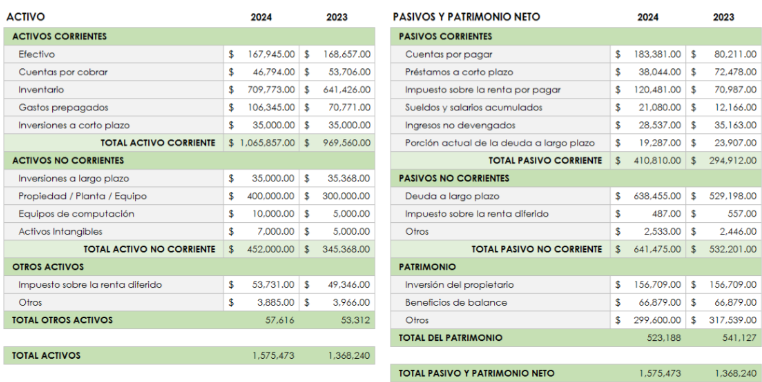
\includegraphics[width=15cm]{./assets/balance.png}
% \end{center}
% \begin{center}
%   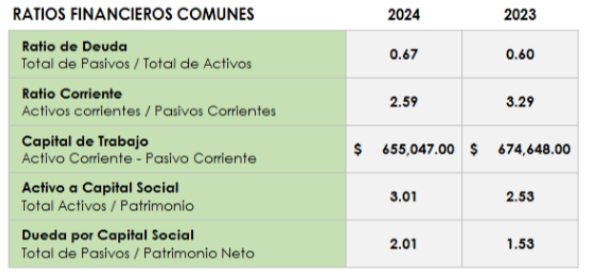
\includegraphics[width=8cm]{./assets/ratios_financieros.png}
% \end{center}

\newpage
\section{Gestión de Ventas}

La gestión de ventas de Nvidia se centra en la identificación de oportunidades de venta, la prospección de clientes, la presentación de propuestas comerciales, el cierre de ventas y el seguimiento postventa. La empresa utiliza un enfoque consultivo para la venta de sus productos y servicios, que se basa en la comprensión de las necesidades y deseos de los clientes y en la presentación de soluciones personalizadas que satisfagan sus requerimientos.

NVIDIA además de la mencionada utiliza diversas estrategias específicas para cerrar ventas, estas estrategias están diseñadas para persuadir a los clientes y garantizar que tomen la decisión de compra. 

Algunas de las estrategias más destacadas son: 

\begin{itemize}
  \item \textbf{Ofrecer Valor Tangible y Diferenciación:} Demostraciones Prácticas: NVIDIA organiza eventos, presentaciones y videos donde muestra el rendimiento real de sus productos, como gráficos avanzados, inteligencia artificial o simulaciones en tiempo real. Esto ayuda a los clientes a visualizar el valor que obtendrán. 

  Comparación con la Competencia: Destaca características únicas, como su tecnología RTX para trazado de rayos y la eficiencia energética de sus chips frente a alternativas del mercado. 

  \item \textbf{Paquetes de Valor Añadido:} Incluye Software Complementario: Ofrecen programas como NVIDIA GeForce Experience o herramientas profesionales como Omniverse sin costo adicional, mejorando el valor del producto. 

  Promociones de Juegos y Servicios: En el segmento de gaming, NVIDIA ofrece juegos gratuitos o descuentos en títulos selectos al comprar sus GPUs, haciendo la oferta más atractiva. 

  \item \textbf{Argumentos de Rentabilidad a Largo Plazo:} En el mercado empresarial, NVIDIA enfatiza el retorno de inversión (ROI). Por ejemplo, en sus GPUs para inteligencia artificial o centros de datos, argumentan que sus soluciones reducen costos operativos debido a su alta eficiencia y rendimiento.  
  En gaming, destacan la durabilidad y soporte continuo, mostrando que sus productos mantienen su relevancia durante años. 

  \item \textbf{Creación de Escasez y Exclusividad:} NVIDIA a menudo utiliza la estrategia de escasez durante lanzamientos de productos, limitando la disponibilidad inicial para crear un sentido de urgencia en los consumidores. 
  Resalta la exclusividad de características como el soporte RTX en juegos seleccionados, creando la percepción de que los clientes obtendrán algo único. 
  
  \item \textbf{Construcción de Relación y Confianza:} Atención Personalizada: En ventas corporativas, NVIDIA trabaja directamente con empresas para entender sus necesidades y diseñar soluciones personalizadas (como arquitecturas específicas para IA o simulación). 

  Programas de Soporte: Ofrecen soporte técnico sólido y continuo, asegurando que los clientes tengan confianza en la marca al momento de la compra. 
  
  \item \textbf{Apoyo de Socios y Distribuidores:} Apalancamiento de Canales de Ventas: Trabajan estrechamente con socios minoristas y mayoristas para ofrecer ofertas atractivas y garantizar una experiencia de compra fluida. 

  Entrenamiento para Equipos de Ventas: Capacitan a los representantes de ventas en tiendas para que destaquen los beneficios específicos de sus productos frente a la competencia. 

  \item \textbf{Garantías y actualizaciónes:} Ofrecen garantías sólidas para asegurar la tranquilidad del cliente. Además, destacan el soporte continuo a través de actualizaciones de drivers y software que mejoran el rendimiento con el tiempo. 
  
\end{itemize}

% \begin{center}
%   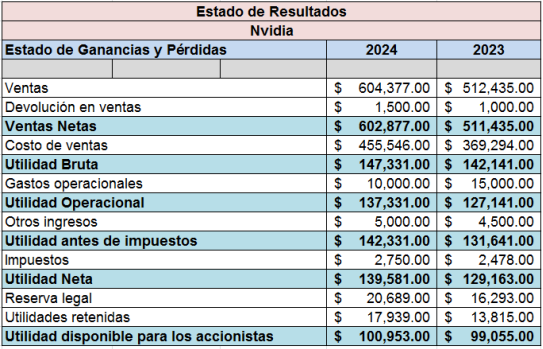
\includegraphics[width=15cm]{./assets/estado_resultados.png}
% \end{center}

\newpage

\section{Gestión del Servicio}

La gestión del servicio al cliente de Nvidia se centra en la atención al cliente, la resolución de problemas y la gestión de reclamos. La empresa se esfuerza por ofrecer una experiencia del usuario excepcional, garantizando que los clientes reciban un servicio de alta calidad que satisfaga sus necesidades y expectativas. Nvidia utiliza una combinación de estrategias para gestionar el servicio al cliente, incluyendo la formación de empleados, la implementación de procesos y procedimientos, la recopilación de feedback y la mejora continua de la calidad del servicio.
  
Algunos indicadores para una correcta gestión del servicio podemos encontrarlos aquí:

\begin{enumerate}
  \item \textbf{Tiempo de respuesta:}
  
  Mide el tiempo que tarda la empresa en responder a las consultas y solicitudes de los clientes.
  
  En ese sentido, Nvidia se esfuerza por responder a las consultas de manera automatizada por chatbots o correos electrónicos, y a las solicitudes de soporte técnico en un plazo de 24 horas.

  \item \textbf{Índice de satisfacción del cliente:}
  
  Mide la satisfacción de los clientes con el servicio recibido, a través de encuestas y feedback.
  
  Nvidia al ser una empresa en su más enfocada al modelo B2B, procura mantener su cartera de clientes satisfecha, ofreciendo soporte técnico especializado y soluciones personalizadas, de hecho, ello hace que algunos de sus productos también sean personalizados.

  \item \textbf{Índice de resolución de problemas:}
  
  Mide la eficacia de la empresa en la resolución de problemas y reclamos de los clientes.
  
  Nvidia se esfuerza por resolver los problemas y reclamos de los clientes de manera rápida y eficiente, garantizando una experiencia positiva en cada interacción. Problemas como la garantía de los productos, la devolución de los mismos, entre otros, son resueltos de manera rápida y eficiente.

  \item \textbf{Índice de fidelización de clientes:} 
  
  Mide la lealtad de los clientes hacia la empresa y sus productos, a través de la repetición de compras y recomendaciones.

  Nvidia tiene una ventaja competitiva en la fidelización de clientes, ya que sus productos son altamente especializados y de alta calidad, lo que genera una lealtad a largo plazo. Además, la empresa ofrece programas de fidelización y beneficios exclusivos para sus clientes.

  Además, Nvidia ofrece a algunos de sus clientes que adquieren productos de alta gama, accesibilidad anticipada a nuevo software basado en inteligencia artificial lo cual les permite tener una ventaja competitiva en el mercado.

  \item \textbf{Índice de calidad del servicio:}
  
  Mide la calidad del servicio ofrecido por la empresa, basado en la precisión, amabilidad y eficiencia de los empleados.

  Nvidia puede calcular este índice en comparación con la calidad de servicio de la competencia, para identificar áreas de mejora y oportunidades de diferenciación. AMD y Intel son sus competidores más cercanos, por lo que la calidad del servicio es un factor clave para mantener su posición de liderazgo en el mercado.

\end{enumerate} 
  
\newpage
\section{Gestión del Personal}

La gestión del personal de Nvidia se centra en la selección, contratación, capacitación, evaluación y desarrollo del personal. La empresa se esfuerza por atraer y retener a los mejores talentos, ofreciendo oportunidades de crecimiento y desarrollo profesional a sus empleados. La gestión del personal de Nvidia se basa en la meritocracia, la transparencia y la equidad, garantizando un ambiente de trabajo inclusivo y colaborativo.

A continuación se presenta un organigrama de la empresa Nvidia:

\begin{center}
  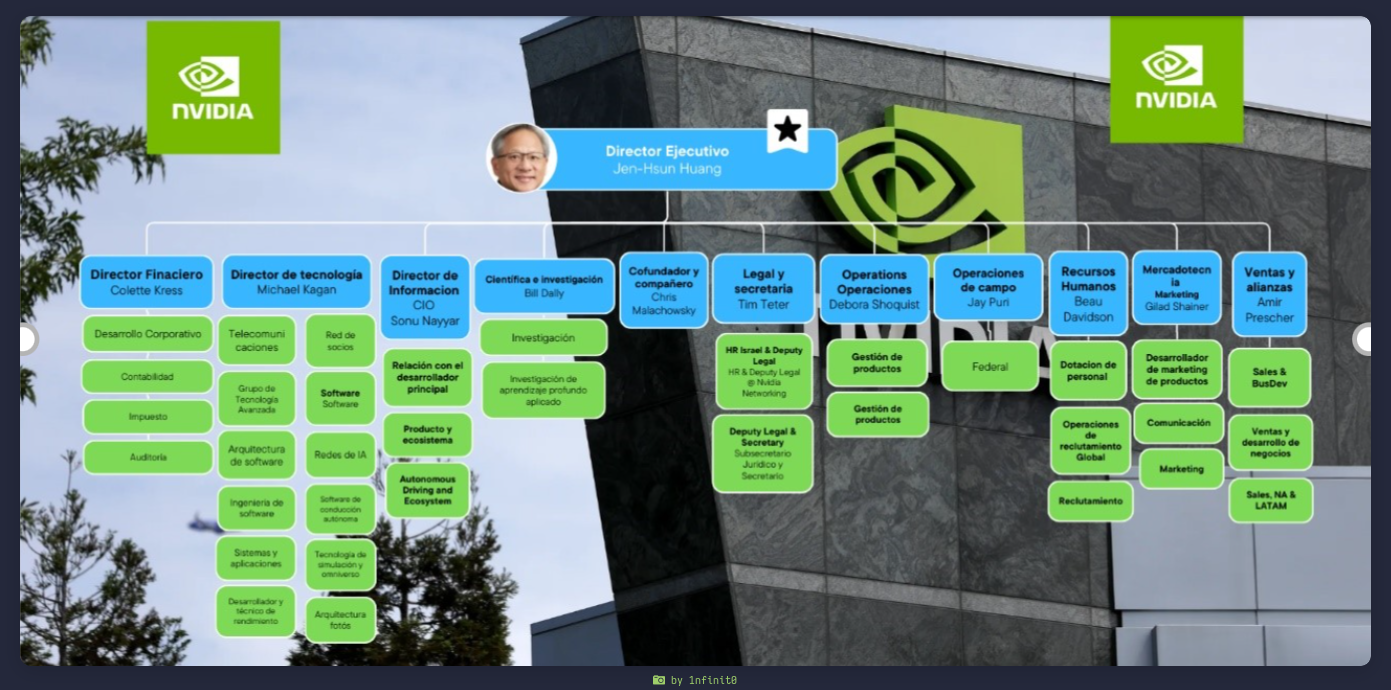
\includegraphics[width=15cm]{assets/forest.png}
\end{center}

\section{Selección del Personal}

La selección del personal es un aspecto clave de la gestión del personal de Nvidia, ya que la empresa busca atraer a los mejores talentos para impulsar su innovación y crecimiento.

\subsection{Sobre la selección del personal}

Nvidia utiliza una combinación de estrategias para seleccionar a los mejores talentos, incluyendo:

\begin{enumerate}
  \item Procesos de selección rigurosos: la empresa utiliza pruebas técnicas, entrevistas y evaluaciones de habilidades para evaluar a los candidatos y garantizar que cumplan con los requisitos del puesto.
  \item Evaluación de competencias: Nvidia evalúa las competencias técnicas y blandas de los candidatos, como la capacidad de resolución de problemas, la creatividad, la comunicación y la colaboración.
  \item Cultura organizacional: la empresa busca candidatos que se ajusten a su cultura organizacional, basada en la innovación, la excelencia y el trabajo en equipo.
  \item Desarrollo profesional: Nvidia ofrece oportunidades de desarrollo profesional y crecimiento a sus empleados, lo que les permite adquirir nuevas habilidades y avanzar en sus carreras.
  \item Experiencia en Investigación y Desarrollo: Nvidia valora la experiencia en investigación y desarrollo de sus empleados, ya que la innovación es un pilar fundamental de su estrategia de negocio.
\end{enumerate}

\section{Retención del Personal}

La retención del personal es crucial para Nvidia, ya que la empresa busca mantener a los mejores talentos y fomentar su desarrollo continuo.

Nvidia utiliza una combinación de estrategias para retener a su personal, incluyendo:

\subsection{Cultura de Trabajo Positiva}

\begin{enumerate}
  \item Ambiente inclusivo: fomenta la diversidad y la inclusión, creando un espacio de trabajo donde todos se sientan valorados y respetados. 
  \item Comunicación abierta: la empresa se esfuerza por mantener una comunicación transparente y honesta con sus empleados, informándoles sobre las estrategias, objetivos y planes de la empresa. 
  \item Trabajo en equipo: promueve la colaboración y el trabajo en equipo, creando un ambiente de apoyo y aprendizaje. 
\end{enumerate}

\subsection{Desarrollo y Crecimiento Profesional}

\begin{enumerate}
  \item Oportunidades de aprendizaje: la empresa ofrece una variedad de cursos, talleres y programas de formación para que sus empleados puedan desarrollar nuevas habilidades y conocimientos.
  \item Planes de carrera: define rutas de crecimiento y ascenso de manera interna, con objetivos y metas para que los empleados puedan seguir con sus carreras.
  \item Programas de rotación: permite que sus empleados experimenten diferentes áreas y roles ampliando su experiencia y conocimiento dentro de la empresa.
\end{enumerate}

\subsection{Reconocimiento y Recompensas}

\begin{enumerate}
  \item Programas de incentivos: ofrece un bono/recompensa por su desempeño, logros y contribuciones al equipo.
  \item Beneficios competitivos: ofrece paquetes de beneficios incluyendo seguro médico, dental y de bienestar.
  \item Reconocimiento público: celebra los logros de sus empleados y reconoce el esfuerzo e impacto en la empresa.
\end{enumerate}

\subsection{Liderazgo}

La empresa se enfoca en desarrollar a líderes que den soporte (apoyo) a los empleados que recién se van a integrando a la empresa para que los inspiren y motiven a seguir con su trabajo del día a día. Por ello tenemos que mantener una comunicación abierta y fluida entre los líderes y los empleados. Y así puedan desarrollar su talento nato dentro de la empresa, brindando oportunidades de crecimiento y aprendizaje.

\subsection{Onboarding}

Nvidia ofrece un programa de inducción integral para los nuevos empleados, para que introduzcan su cultura, valores y expectativas sobre el área en el que están laborando. Luego el empleado es asignado con un colaborador capacitado para que lo guie y despeje sus dudas acerca de la empresa o del puesto, además para que se incluyan con los demás, la empresa organiza actividades de integración.

Nvidia, al implementar estas estrategias, crea un ambiente de trabajo atractivo y positivo que ayuda a retener a su personal. Su enfoque en el desarrollo, el reconocimiento y la cultura de trabajo les permite no solo atraer talento, sino también retenerlo a largo plazo.

\newpage

\section{Iniciativas de TI para optimizar la eficiencia en NVIDIA}

La gestión de TI juega un papel crucial en la eficiencia de cualquier empresa moderna. Para optimizar esta eficiencia, se deben implementar iniciativas estratégicas que aprovechen las últimas tecnologías y tendencias. A continuación, se proponen algunas iniciativas de TI con un enfoque en la productividad, la colaboración y la reducción de costes: 

\begin{enumerate}
  \item Automatización de procesos:
  \begin{itemize}
    \item Implementación de RPA: Automatizar tareas repetitivas y de bajo valor como la introducción de datos, la gestión de facturas o el envío de correos electrónicos.
    \item Integración de API: Permitir que diferentes sistemas de software se comuniquen entre sí, eliminando la necesidad de introducir datos manualmente y mejorando la fluidez de la información.
    \item Utilización de IA para la automatización: Implementar soluciones de IA para automatizar tareas más complejas como la gestión de inventarios, la predicción de la demanda o la detección de fraudes.
  \end{itemize}
  \item Mejora de la colaboración y la comunicación:
  \begin{itemize}
    \item Adopción de plataformas de colaboración en la nube: Implementar plataformas como Microsoft Teams, Slack o Google Workspace para facilitar la comunicación interna, la gestión de proyectos y la colaboración en tiempo real.
    \item Implementación de herramientas de videoconferencia: Facilitar la comunicación remota y la realización de reuniones virtuales con herramientas como Zoom, Google Meet o Microsoft Teams.
    \item Utilización de herramientas de gestión de proyectos: Implementar herramientas como Asana, Trello o Jira para organizar tareas, establecer plazos y mejorar la visibilidad del progreso de los proyectos.
  \end{itemize}
  \item Optimización de la infraestructura tecnológica:
  \begin{itemize}
    \item Migración a la nube: Trasladar aplicaciones y datos a la nube para reducir los costes de infraestructura, mejorar la escalabilidad y aumentar la seguridad.
    \item Implementación de soluciones de seguridad en la nube: Proteger los datos y sistemas de la empresa con soluciones de seguridad avanzadas como firewalls, antivirus y sistemas de detección de intrusiones.
    \item Actualización del hardware y software: Mantener los sistemas actualizados con las últimas versiones para mejorar el rendimiento, la seguridad y la compatibilidad.
  \end{itemize}
  \item Análisis de datos y toma de decisiones:
  \begin{itemize}
    \item Implementación de herramientas de análisis de datos: Utilizar herramientas como Power BI, Tableau o Qlik Sense para analizar datos, identificar tendencias y tomar decisiones más informadas.
    \item Utilización de dashboards y reportes: Visualizar datos clave de la empresa en dashboards y reportes para facilitar la toma de decisiones y el seguimiento del progreso.
    \item Integración de datos de diferentes fuentes: Combinar datos de diferentes sistemas para obtener una visión más completa del negocio y mejorar la toma de decisiones.
  \end{itemize}
  \item Gestión del cambio y capacitación:
  \begin{itemize}
    \item Comunicación clara y constante: Informar a los empleados sobre las nuevas iniciativas de TI, sus beneficios y cómo utilizar las nuevas herramientas.
    \item Capacitación y entrenamiento: Ofrecer programas de capacitación para que los empleados puedan utilizar las nuevas herramientas y tecnologías de forma efectiva.
    \item Apoyo y asistencia: Proporcionar asistencia técnica a los empleados para resolver problemas y asegurar una transición suave a las nuevas herramientas.
  \end{itemize}
  \item Auditoría y evaluación periódica:
  \begin{itemize}
    \item Realizar auditorías periódicas de la infraestructura de TI: Identificar áreas de mejora, actualizar los sistemas y garantizar que la tecnología se está utilizando de forma eficiente.
    \item Evaluar el impacto de las iniciativas de TI: Medir el retorno de la inversión (ROI) de las iniciativas de TI y ajustar las estrategias según sea necesario.
  \end{itemize}
  \item Consideraciones adicionales:
  \begin{itemize}
    \item Eficiencia energética: Implementar soluciones de eficiencia energética en la infraestructura de TI para reducir el consumo de energía y los costes operativos.
    \item Seguridad de la información: Implementar medidas de seguridad robustas para proteger los datos de la empresa de accesos no autorizados, ataques cibernéticos y otros riesgos.
    \item Cumplimiento normativo: Asegurar que la infraestructura de TI cumple con las normas y regulaciones relevantes para la industria y el sector.
  \end{itemize}
\end{enumerate}

\section{Gestión de Investigación y Desarrollo (I + D)}

Para Nvidia, una empresa que se encuentra a la vanguardia de la tecnología, la innovación es clave para mantener su liderazgo en áreas como los gráficos por computadora, la inteligencia artificial (IA), la computación de alto rendimiento (HPC) y las plataformas de videojuegos. A continuación, se presentan algunas estrategias innovadoras que podrían seguirse para fomentar aún más la innovación en Nvidia: 

\textbf{Desarrollo de Arquitecturas Híbridas para el Edge Computing y 5G}

A medida que las redes 5G y la computación en el borde (edge computing) continúan creciendo, Nvidia podría centrarse en la creación de arquitecturas híbridas que permitan la integración de sus potentes GPUs con dispositivos de edge computing. Esto permitiría una mayor capacidad de procesamiento en tiempo real, reduciendo la latencia y mejorando el rendimiento de las aplicaciones en áreas como vehículos autónomos, IoT industrial y videojuegos en la nube.

\textbf{Colaboración con la Industria Automotriz para la Conducción Autónoma}

Nvidia ya está presente en el ámbito de los vehículos autónomos con su plataforma NVIDIA DRIVE. Sin embargo, podría avanzar en esta área con nuevas innovaciones:
\begin{itemize}
  \item Desarrollando soluciones más integradas y escalables para diferentes tipos de vehículos (desde automóviles hasta camiones y drones).
  \item Impulsando la colaboración con empresas de transporte y logística para crear soluciones de movilidad inteligente.
  \item Explorando el uso de simulaciones virtuales en entornos urbanos para mejorar las capacidades de los vehículos autónomos.
\end{itemize}

\textbf{Explorar Nuevas Aplicaciones de la Realidad Aumentada (AR) y Realidad Virtual (VR)}

La realidad aumentada y la realidad virtual son áreas con mucho potencial en sectores como la educación, la medicina y la capacitación empresarial. Nvidia podría expandir su presencia en estos sectores creando:
\begin{itemize}
  \item Soluciones para entornos inmersivos de capacitación utilizando AR y VR para el sector empresarial y educativo.
  \item Plataformas basadas en GPU para mejorar el rendimiento de las aplicaciones de AR/VR, optimizando la experiencia del usuario.
  \item Colaboraciones con empresas tecnológicas para la creación de dispositivos portátiles (como gafas AR o sistemas VR avanzados) optimizados para la interactividad de alto rendimiento.
\end{itemize}

\textbf{Incorporar Blockchain para la Seguridad en IA y Datos}

Dado el crecimiento de la inteligencia artificial y la gestión de datos, Nvidia podría explorar la integración de blockchain para mejorar la seguridad y transparencia en sus plataformas. Esto sería especialmente relevante para:
\begin{itemize}
  \item Garantizar la protección de los datos en las plataformas de IA utilizadas para la salud, la seguridad pública o los servicios financieros.
  \item Desarrollar sistemas que permitan un entrenamiento descentralizado de modelos de IA, permitiendo la colaboración sin compartir datos sensibles directamente.
\end{itemize}

\textbf{Expandir el Uso de sus GPUs en Sectores no Tecnológicos}

Finalmente, Nvidia podría explorar aplicaciones innovadoras de sus GPU en sectores no tradicionales, como:
\begin{itemize}
  \item Biotecnología y genómica, usando sus potentes GPUs para acelerar investigaciones en el campo de la salud y la biomedicina.
  \item Agricultura inteligente, mediante el uso de IA y sus GPU para optimizar la gestión de cultivos, el uso de recursos y la predicción de patrones climáticos.
\end{itemize}

\section{Gobierno corporativo}
El gobierno corporativo de Nvidia se fundamenta en principios de responsabilidad, transparencia, equidad y rendición de cuentas, asegurando una gestión ética y eficaz. Los órganos clave incluyen la Junta Directiva, responsable de las decisiones estratégicas, y los Comités de Auditoría y Riesgos, que supervisan el control interno y la gestión de riesgos.

\subsection{Ética Empresarial}

La ética empresarial en Nvidia se basa en un conjunto de valores y principios que guían el comportamiento y las decisiones dentro de la organización. Su importancia radica en generar confianza, contribuir a la reputación corporativa, prevenir fraudes y promover un entorno laboral positivo. Se manifiesta en tres dimensiones: individual (conducta de los empleados), corporativa (cultura organizacional) y social (compromiso con la sociedad).

\subsection{Control Interno y Gestión de Riesgos}

El control interno es un sistema diseñado para asegurar la efectividad operativa, la integridad financiera y el cumplimiento normativo. La gestión de riesgos implica identificar, evaluar y mitigar riesgos potenciales. Ambos procesos se complementan para proteger los activos de la empresa y garantizar el cumplimiento de objetivos. Los beneficios incluyen una toma de decisiones mejorada, mayor eficiencia operativa y protección de la reputación.

\subsection{Responsabilidad Social Empresarial (RSE)}

La RSE permite a Nvidia contribuir al bienestar social y ambiental, fortaleciendo su reputación y éxito a largo plazo. A través de la RSE, la empresa puede mejorar su competitividad, atraer inversores y fomentar la innovación. Las áreas de enfoque incluyen la responsabilidad ambiental, social y económica, con beneficios como el aumento de la competitividad y la atracción de inversores conscientes.

\subsection{Prácticas Fundamentales para el Buen Funcionamiento de la Empresa}

\begin{itemize}
  \item \textbf{Innovación Continua:} Es esencial para mantenerse competitivo en sectores dinámicos como la tecnología, asegurando que la empresa se adapte y lidere los avances del mercado.
  \item \textbf{Cultura Inclusiva:} Promueve un entorno de trabajo colaborativo y diverso, esencial para motivar al talento y generar ideas innovadoras.
  \item \textbf{Responsabilidad Social:} Refleja el compromiso de Nvidia con la sostenibilidad y el impacto positivo, mejorando su reputación y atrayendo clientes responsables.
  \item \textbf{Gestión de Riesgos:} Previene problemas financieros, legales y operativos, asegurando estabilidad y éxito a largo plazo.
  \item \textbf{Alianzas Estratégicas:} Amplían las capacidades de la empresa y fomentan la creación de nuevas oportunidades en el mercado.
  \item \textbf{Atención al Cliente:} Fortalece la relación con los consumidores, asegurando satisfacción y fidelidad, lo que es clave para el crecimiento sostenido.
\end{itemize}


\section{Conclusiones y recomendaciones}

Es posible concluir que Nvidia es una empresa líder en innovación tecnológica, con una sólida gestión empresarial y un enfoque en la responsabilidad social y la sostenibilidad. Su estrategia de marketing mix, que incluye productos de alta calidad, precios premium, una amplia red de distribución y promociones efectivas, ha contribuido significativamente a su éxito en el mercado. La empresa ha demostrado una gestión financiera sólida, con un balance general y un estado de resultados que reflejan un crecimiento constante y una rentabilidad sostenida. Además, la gestión del personal de Nvidia, que se centra en la selección, retención y desarrollo de talento, ha creado una cultura organizacional inclusiva y colaborativa. Nvidia ha mostrado un compromiso con la responsabilidad social y la sostenibilidad, implementando prácticas que contribuyen al bienestar social y ambiental. Esto no solo mejora su reputación, sino que también atrae a inversores y clientes conscientes.

\subsection{Conclusiones}

1. \textbf{Liderazgo en Innovación:} Nvidia ha demostrado ser un líder en innovación tecnológica, especialmente en el desarrollo de GPUs y soluciones de inteligencia artificial. Su enfoque en la investigación y desarrollo ha permitido a la empresa mantenerse a la vanguardia de la industria tecnológica.

2. \textbf{Diversificación de Productos:} La diversificación de productos de Nvidia, que abarca desde GPUs para gaming hasta soluciones de IA y computación en la nube, ha fortalecido su posición en el mercado y ha abierto nuevas oportunidades de crecimiento.

3. \textbf{Estrategia de Marketing Efectiva:} La estrategia de marketing mix de Nvidia, que incluye un enfoque en productos de alta calidad, precios premium, una amplia red de distribución y promociones efectivas, ha contribuido significativamente a su éxito en el mercado.

4. \textbf{Gestión Financiera Sólida:} Nvidia ha demostrado una gestión financiera sólida, con un balance general y un estado de resultados que reflejan un crecimiento constante y una rentabilidad sostenida. Los indicadores financieros muestran una empresa bien posicionada para enfrentar desafíos futuros.

5. \textbf{Gestión del Personal y Cultura Organizacional:} La gestión del personal de Nvidia, que se centra en la selección, retención y desarrollo de talento, ha creado una cultura organizacional inclusiva y colaborativa. Esto ha permitido a la empresa atraer y retener a los mejores talentos en la industria.

6. \textbf{Responsabilidad Social y Sostenibilidad:} Nvidia ha mostrado un compromiso con la responsabilidad social y la sostenibilidad, implementando prácticas que contribuyen al bienestar social y ambiental. Esto no solo mejora su reputación, sino que también atrae a inversores y clientes conscientes.

\subsection{Recomendaciones}

1. \textbf{Fortalecer la Innovación:} Continuar invirtiendo en investigación y desarrollo para mantener el liderazgo en innovación tecnológica. Explorar nuevas áreas de aplicación para sus tecnologías, como la biotecnología y la agricultura inteligente.

2. \textbf{Expandir la Presencia en Mercados Emergentes:} Ampliar la presencia de Nvidia en mercados emergentes, donde hay un gran potencial de crecimiento. Adaptar las estrategias de marketing y distribución para satisfacer las necesidades específicas de estos mercados.

3. \textbf{Mejorar la Gestión de Riesgos:} Fortalecer los procesos de gestión de riesgos y control interno para mitigar posibles amenazas y garantizar la estabilidad a largo plazo. Implementar tecnologías avanzadas de seguridad, como blockchain, para proteger los datos y sistemas de la empresa.

4. \textbf{Fomentar la Diversidad e Inclusión:} Continuar promoviendo la diversidad y la inclusión en el lugar de trabajo. Implementar programas de capacitación y desarrollo que fomenten un ambiente de trabajo inclusivo y colaborativo.

5. \textbf{Optimizar la Eficiencia Operativa:} Implementar iniciativas de TI que optimicen la eficiencia operativa, como la automatización de procesos y la migración a la nube. Utilizar herramientas de análisis de datos para mejorar la toma de decisiones y la gestión de recursos.

6. \textbf{Fortalecer la Responsabilidad Social:} Continuar implementando prácticas de responsabilidad social y sostenibilidad. Colaborar con organizaciones y comunidades para desarrollar proyectos que generen un impacto positivo en la sociedad y el medio ambiente.

En resumen, Nvidia ha demostrado ser una empresa líder en innovación tecnológica y gestión empresarial. Sin embargo, para mantener su posición competitiva y seguir creciendo, es crucial que continúe invirtiendo en investigación y desarrollo, expanda su presencia en mercados emergentes, fortalezca la gestión de riesgos y fomente la diversidad e inclusión en el lugar de trabajo. Además, debe seguir implementando prácticas de responsabilidad social y sostenibilidad para contribuir al bienestar social y ambiental.


\newpage

\begin{thebibliography}{9}

  \bibitem{paucar} 
  Paucar J. (2019) Evolución de las 4P´s o Marketing Mix. Recuperado de: \url{https://www.gestiopolis.com/evolucion-de-las-4ps-o-marketing-mix/}

  \bibitem{rojas}
  Rojas Z. (2017) La Gestión de Ventas y Rentabilidad. Recuperado de: \url{https://www.gestiopolis.com/la-gestion-ventas-la-rentabilidad/}

  \bibitem{pineiro}
  Piñeiro A. Varela J. Rail A. (2006) El análisis de importancia-valoración aplicado a la gestión de servicios. Recuperado de: \url{https://www.gestiopolis.com/el-analisis-de-importancia-valoracion-aplicado-a-la-gestion-de-servicios/}

  \bibitem{sonderegger}
  Sonderegger P. (2020) Cómo utilizar el Business Model Canvas (Lienzo de Modelo de Negocio) para reducir el riesgo. Recuperado de: \url{https://raia.revistasuai.ar/index.php/raia/article/view/22/52}

\end{thebibliography}

  
\end{document}